For a quantum computer, multiple qubits are needed that are capable of interacting with each other. This is done by making a 2D aray of optical tweezers described in \cref{ch:tweezer}. One of these methods is to let the laser beam refract off a sound wave in a crystal in a acoustic optical deflector. By using 2 of these devices, 2D arrays of Rydberg atoms have been realized in \cite{Madjarov2020}.

This work will make use of another method, a spatial light modulator. This method was proven to work by several groups, one of which the \textit{Schreck} group.

\section{The Spatial Light Modulator}

A spatial light modulator (SLM) can manipulate properties of light like amplitude, phase and polarization. The type of SLM we use is a phase-only SLM, so it can not do amplitude modulation. It does this by deploying a large array of pixels, where each individual pixel has a liquid crytal in it. The orientation of the crystal will change the refractive index because of the birefringence effect. The pixelated display is manufactured on a layer of silicon to address the voltage of each cell invididually. Therefore, this type of SLM is said to use liquid crytal on silicon or LCoS technology. A sketch of the SLM pixels is shown in \cref{fig:LCoS}.

The working principle of this type of SLM has been documented extensively within the CQT group at TU/e, for example by \cite{Dijk2012,Bijnen2013}. A brief review of the working principle of the SLM is presented here.

\begin{figure}
    \centering
    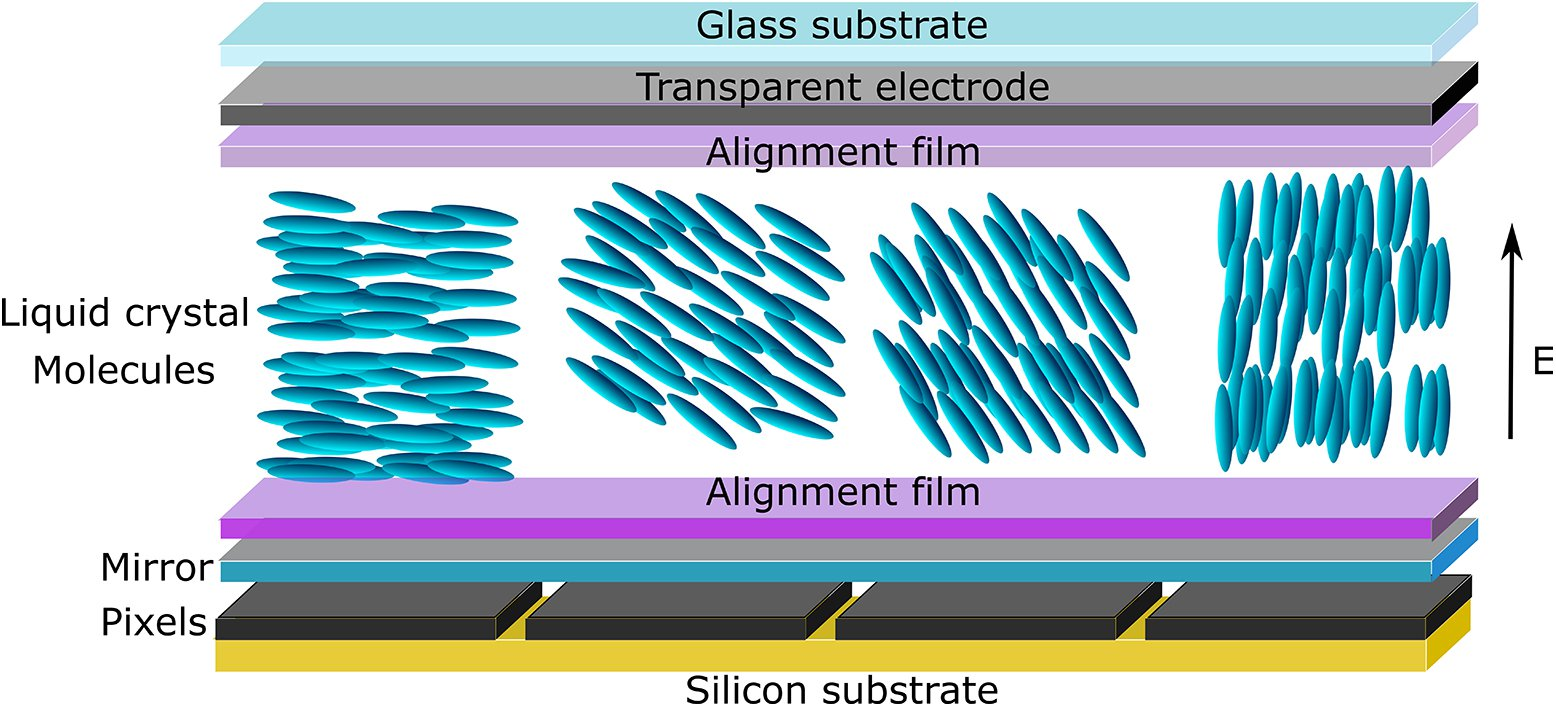
\includegraphics[width=7cm]{figures/LCoS.png}
    \caption{The orientation of the liquid crystal cells changes as a function of the applied electric field $E$.}
    \label{fig:LCoS}
\end{figure}

\section{Phase Modulation}

We consider an ensemble consisting of the SLM and a perfect lens with focal length $f$. We define two cartesian coordinate systems: the SLM plane by $\{x',y'\}$ and the focal plane of the lens by $\{x,y\}$. The situation is sketched in \cref{fig:SLMLens}

\begin{figure}
    \centering
    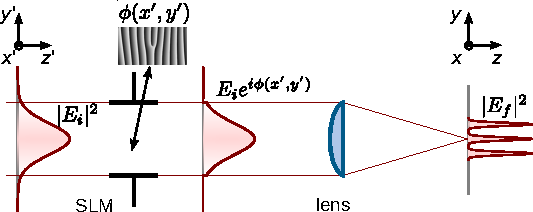
\includegraphics[width = 12cm]{figures/SLMfigure.pdf}
    \caption{Field with intensity distribution $|U_i|^2$ impinging on the SLM, which due to its finite size acts as an aperture. The lens makes the resulting image $|U_f|^2$ in its focal plane. Also shown: two cartesian coordinate systems in the SLM and focal plane. Not to scale. Adapted from \cite{Labuhn2016}.}
    \label{fig:SLMLens}
\end{figure}

The SLM imprints a phase pattern $\phi(x',y')$ onto the impinging gaussian laser $U_i(x',y')$ According to Fourier optics, the complex amplitude in the focal plane of the lens $U_f(x,y)$ is given by the 2D spatial fourier transform, with spatial frequencies $x'/\lambdaup f$ and $y'/\lambdaup f$ \cite{Bijnen2015}

\begin{equation}\label{FourierLens}
    U_f(x,y) = \mathscr{F} \big\{ U_i(x', y')e^{i \phi(x',y')} \big\} \left(\frac{x'}{\lambdaup f},\frac{y'}{\lambdaup f}\right),
\end{equation}

where $\mathscr{F}\{\cdot\}$ denotes the Fourier transform. A derivation of \cref{FourierLens} can be found in \cite{Dijk2012,Bijnen2013}. In practice, we are interested by the intensity distribution, which we find from the norm of \cref{FourierLens}: $I_f(x,y) = \left|U_f(x,y)\right|^2$

In reality, the SLM has a finite amount of pixels and cannot make continuous holograms $\phi(x,y)$. As long as the pixel size is very small compared to the size of the entire chip, we can approximate the incoming light as a series of delta peaks \cite{Bijnen2013,Labuhn2016}, each having amplitude and phase contributions $U_i$ and $\phi_{kl}$ respectively, where $k,l$ sum over the pixels in $x$ and $y$:

\begin{equation}\label{LightDiscretization}
    U(x',y') \approx \sum_{k,l} \delta(x-x_k, y-y_l)  U_i(x_k,y_l) e^{i \phi_{kl}}
\end{equation}

We can use the a nice property of the delta function to compute its fourier transform: \cref{LightDiscretization} 

\begin{equation}\label{DFT}
    U^f(m \Delta_x, n \Delta_y) = \sum_{k,l} U(k \Delta_x',l \Delta_y') e^{i \phi_{kl}} e^{-i 2\pi (km/N_x+ln/N_y)}
\end{equation}

The superscript $U^f$ is used to indicate the variable is now a discrete array and no longer a conituous function. \cref{DFT} is the discrete Fourier transform, and it can be evaluated on a computer using a fast fourier transform algorithm. 

\begin{equation}\label{DFTshort}
    U^f_{nm} = \text{DFT}\{U^i\}_{nm}
\end{equation}

The subscript $U_{nm}$ is used to indicate it is defined on the discrete grid in the focal plane. The discrete Fourier transform is implemented on computers in so called fast fourier transform (FFT) algorithms. 



\section{Finding the Hologram}\label{IFTA}

$U_f$ and $U_i$ are known in an experiment. Thus if one finds the right phase pattern or hologram $\phi(x,y)$, any intensity distrubution can be found from \cref{FourierLens}. But a single inverse inverse fast Fourier transform (IFFT) will not suffice, because this will not modulate the phase contributions of the invididual pixels $\phi_{kl}$ but also the amplitude contributions, which a phase-only SLM, by far the most commonly used SLM, cannot do. 

Instead, a set of algorithms known as inverse Fourier transform algorithms (IFTA) were pioneered by \cite{Hirsch1971} and adapted by \cite{Gerschberg1972} to tackle this task. The goal of the algorithm is to find a phase pattern for the SLM, such that in the focal plane of the lens, the light intensity $I_m = |V_m|^2$ in invidual spots $m$ is optimized in terms of parameters diffraction efficiency efficiency $e$ and uniformity of the spots $u$ \cite{DiLeonardo2007}:

\begin{equation}\label{EfficiencyUniformity}
    e = \sum_m |V_m|^2, \quad u= 1-\frac{\text{max}(|V_m|^2)-\text{min}(|V_m|^2)}{\text{max}(|V_m|^2)+\text{min}(|V_m|^2)}
\end{equation}

These are theorical quantities and not actually measured. The algorithm works essentially by virtually propagating light back and forward in iterations acoording by computing FFT and IFFT's, applying constraints in the focal and SLM plane in each iteration. 




In order to overcome this issue, after the inverse FFT we replace the computed complex amplitude by our incident amplitude $PU_0$ and we compute its FFT, returning again to the focal plane. Here, we replace the obtained obtained complex amplitude for the desired amplitude $|U(x,y)|^2$. This process is iterated several times until convergence is reached. This family of algorithms is refered to as an inverse Fourier transform algorithm (IFTA) and essentially consists of virtually propagating light back and forward between the input and focal planes. 

IFTA algorithms were pioneered in\cite{Hirsch1971} and adapted for phase retrieval by \cite{Gerschberg1972}. The implementation of the IFTA algorithm was done by \cite{Bijnen2013,Bijnen2015}. It was adapted to achieve better convergence by defining a signal window, within it the desired pattern is made. Outside of this window, the amplitude is unconstrained. This relaxiation of constraints allows for better convergence of the desired pattern, at the cost of energy lost outside of the window \cite{Bijnen2013,Bijnen2015}.

\section{Operating the SLM}

The algorithm as explained in \cref{IFTA} was implented in software by \cite{Bijnen2015}. The input intensity $|PU_0|^2$ is assumed to be a plane wave. Using the SLM is explained here. The SLM will inevitably lose power due to several processes. These are explained here. 

\subsection{Diffraction}

Diffraction. The SLM is a device consisting of individual pixels. Therefore, it is essentially a 2D diffraction grating, and light will diffract in several directions. In 1D, we know that according to diffraction theory the diffraction angle maxima $\theta_m$ from a plane wave incident at $\theta_i$ occur at $\theta_m = \arcsin(\sin\theta_i - m\lambdaup/d)$, where $m$ is the order of diffraction and $d$ the pixel pitch. We are interested in the light in the $m=0$ diffracton order, other orders are spatially filtered out and unused.

\subsection{Zeroth Order}

Light can reflect on the spacings between the pixels. Also, it can reflect off of the electrodes at the back of the device. All of this undiffracted light is focussed onto the optical axis by the objective. As a result, the optical axis unusable to shape light and we have to seperate our modulated light from this 'zeroth order peak'. This is done by superimposing a linear phase on top of the SLM phase pattern. Because the phase is computed modulo 2$\pi$ the resulting pattern is a blazed grating. Light from the higher diffraction orders and zeroth order peak can be blocked by an iris in the focal plane of an intermediaty lens. 
    
\subsection{Finite aperture size}

In order to employ the maximum amount of pixels the SLM has to offer, and therefore the maximum drawing area in the focal plane of the Fourier lens, all of the pixels should be illuminated. However, because the incident beam is described by a gaussian, this will lead to power loss as a result of light not falling on the active pixel area. 
    
We can estimate this power loss by shining a Gaussian beam $G(x,y)$ of width $w(z)$ and power $P_0$ onto a rectangular aperture of dimensions $(2S_x, 2S_y)$ where $S_{x,y}$ are the semi-widths of the aperture. The relative power transmission $P/P_0$ can be found by integrating the intensity of the beam \cref{GaussianBeamIntensity} in cartesian coordinates over the aperture

\begin{equation}\label{RectAperturePower}
    \frac{P}{P_0} =
    \iint I(x,y) dA=
    \text{Erf}\left(\frac{\sqrt{2}S_x}{w(z)}\right) \text{Erf}\left(\frac{\sqrt{2}S_y}{w(z)}\right)
\end{equation}

where Erf($\cdot$) denotes the error function. The optimum incident beam size $w(z)$ is thus a compromize between drawing area and power efficiency. We chose $w(z) \approx S_{x}$, specifically $w(z) = 4.8$ mm and $S_x = 4.9$ mm. 

\subsection{Reflectivity}

As can be seen in \cref{fig:LCoS}, the light will back reflect at after passing through the liquid crystal. This back plate will have a non-perfect anti relection coating, leading to some light being absorbed. 


\section{Calibration}

We know that the phase pattern of the SLM is realized by the birefringence effect. However, it turns out the phase retardation as a function of the applied voltage is non-linear. Additionally, the surface of the SLM is not fully flat, introducing a small aberration. Both of these effects differ for indiviual SLM units, even for the same model. Therefore, here we will briefly review how to calibrate the SLM to account for these two effect.s 

\subsection{Electro-Optic Response}

The goal of the calibration of the phase as a function of applied voltage (electro-optic response) is to 

\begin{enumerate}
    \item Achieve a linear electric-optic response. 
    \item Ensure the phase is modulate by a full wave $2\pi$ spanning the minimum to the maximum grey level. 
\end{enumerate}

\subsection{Optical flatness correction}

Because of the silicon producetion process, the chip is not completely flat. The optical flatness of SLM was measured to be $0.18\lambdaup$ by manufacturer Meadowlark. Additionally, the manufacturer measured the shape of the correction using Michelson interferometry. By substracting this measured non-flatness from the calculated phase pattern, this effect can be corrected. 


\section{Arrays of tweezers}

\subsection{Array Spacing}

Because of the properties of the Fourier transform, the smallest possible 

\subsection{Spot Detection}

We make an arbitrarily sized array of optical tweezers. For detecting maxima locations, we could simply set pixels above a certain count threshold as a maxima. The disadvantage of this is that a noisy pixel could be detected as a spot, which would hinder analysis. 

To combat this, we first convolute the image with a Laplacian of Gaussian filter, which first smoothes the image to reduce noise. Subsequently it computes the 2D laplacian to detect edges. If this second derivative is above a certain threshold, we detect the edge as a spot. If the detected amount of spots is not the expected amount, we can easily tune the threshold. The camera image is cropped into regions of interest around the spots marked by the Laplacian of Gaussian filter. 

\subsection{Spot Fitting}

Our tweezers should be described by \cref{FourierBesselAperture}. However, because of a lack of an analytic expression this is not the most convenient. \cref{FourierBesselAperture} can closely be resembled by a Gaussian. We will therefore use the following function for fitting spots numbered $k$

\begin{equation}\label{2DGaussian}
    G_k(x,y) = U_k \exp{\left(-\frac{(x_k-x_{k,0})^2}{2\sigma_{k,x}^2}\right)}
    \exp{\left( \frac{-(y_k-y_{k,0})^2}{2\sigma_{k,y}^2} \right)}
\end{equation}

Here $U$ is the 'trap depth', $x,y$ are the cartesian coordinates in the camera frame and $x_0,y_0$ is the center of the spot. Lastly $\sigma_{x,y}$ are standard deviations in $x$ and $y$. In principle, because the limiting aperture in the system is a circular aperture, the spots should be more or less symmetric and $\sigma_x\approx \sigma_y$ which we confirmed. We find the $1/e^2$ waist $w_k=\sigma_{k,x}+\sigma_{k,y}$. 